% ===========================================================================
%  ISBI submission -- working file.  EDIT THIS FILE (and sections/).
%
%  spconf.sty and IEEEbib.bst are the official ISBI style files and must NOT
%  be edited.
%
%  HOW IT IS ORGANISED
%    1. Switches      -- draft mode on/off, one line
%    2. Numbers       -- every measured number in the paper, defined once,
%                        each with the results file it came from
%    3. Front matter  -- title, authors
%    4. Sections      -- one file each, in sections/, pulled in by \input
%                        below.  The prose, the figures, the tables and each
%                        section's page budget live in those files.
%    5. Ethics        -- REQUIRED by ISBI, see README; sections/6-compliance
%
%  WHY THE NUMBERS ARE HERE AND NOT IN THE SECTIONS.  A number that appears
%  twice in a paper will eventually disagree with itself.  Change it in the
%  \newcommand block and every occurrence follows.  The comment after each
%  one names the file it was measured in, so a reviewer question can be
%  answered in one grep.
%
%  PROPOSED NARRATIVE (rearrange freely -- this is a suggestion, not a
%  decision).  Section 2 shows a failure the field's metrics cannot see,
%  Section 3 shows that the obvious fix -- adopt ERL -- does not work off the
%  shelf because the reference implementation is under-specified, and
%  Section 4 gives the specification that makes it usable.  The alternative
%  running order, recommended in stage-report/ERL_thesis.md section 5, opens
%  with the reference implementation instead.  Pick one before writing prose.
%  Reordering is now a matter of reordering the \input lines.
% ===========================================================================
\documentclass{article}
\usepackage{spconf,amsmath,graphicx}
\usepackage{booktabs}
\usepackage{xcolor}
\usepackage{enumitem}
\setlist{nosep, leftmargin=14pt}

% --- 1. SWITCHES -----------------------------------------------------------
% Set to 0 for the version you submit: TODO notes and the word count vanish.
\newif\ifdraft
\drafttrue          % <-- \draftfalse to hide all draft marks

\ifdraft
  \newcommand{\TODO}[1]{\textcolor{red}{\textbf{[TODO: #1]}}}
  \newcommand{\NOTE}[1]{\textcolor{blue}{\small [#1]}}
\else
  \newcommand{\TODO}[1]{}
  \newcommand{\NOTE}[1]{}
\fi

% Draft-only filler, so an unwritten section still shows how much room it has.
%   \FILL{2-4}       lipsum paragraphs 2 to 4  (roughly 100 words each)
%   \FILLS{15}{1-4}  paragraph 15, first four sentences
% Every call vanishes under \draftfalse. Delete each one as you write the real
% prose; the \TODO above it says what that prose has to do.
% The word budgets in the section files assume ~500 words per ISBI column.
% NOT VERIFIED: this machine cannot compile. Check on Overleaf and retune.
\usepackage{lipsum}
\newcommand{\FILL}[1]{\ifdraft\lipsum[#1]\fi}
\newcommand{\FILLS}[2]{\ifdraft\lipsum[#1][#2]\fi}

% --- 2. NUMBERS ------------------------------------------------------------
% Every measured number in the paper. Do NOT type a measurement into the prose
% in sections/ -- use a macro, so one edit moves every occurrence and a
% reviewer's "where does that come from" is answered by one grep.
%
% numbers.tex is GENERATED by exp/paper_figures.py straight out of
% exp/results/. Regenerate it (and the figures and tables) with:
%     .venv/bin/python exp/paper_figures.py
% Its selftest re-derives erl_spec.txt's printed table from the raw CSV and
% refuses to write anything if the two disagree.
% GENERATED by exp/paper_figures.py -- every macro here is a
% Coverage macros are the mean over ALL twelve cells; the verdict
% files print it per length convention, so they differ by ~1 point.
% measurement read out of exp/results/. Do not edit: edit the
% measurement. Macros NOT in this file (the transcribed reference-
% implementation numbers) stay in main.tex and say so there.

\newcommand{\csImages}{20}
\newcommand{\csCuts}{30}
\newcommand{\csDice}{0.9889}
\newcommand{\csTracedUncut}{98.1}
\newcommand{\csTracedEdgeOff}{98.1}
\newcommand{\csTracedEdgeAny}{59.9}
\newcommand{\csTracedTip}{91.4}
\newcommand{\csTracedMid}{74.0}
\newcommand{\csGap}{17.3}
\newcommand{\csBettiTip}{30.2}
\newcommand{\csBettiMid}{19.8}
\newcommand{\csSplitsMid}{9.4}
\newcommand{\csLoopsMid}{20.7}
\newcommand{\csUnreachMid}{11.1}
\newcommand{\csUnreachTip}{1.4}
\newcommand{\specArms}{10}
\newcommand{\specSeeds}{24}
\newcommand{\specSpreadLo}{38.4}
\newcommand{\specSpreadHi}{41.8}
\newcommand{\specRho}{-0.224}
\newcommand{\specMove}{8}
\newcommand{\txSTARELo}{27.2}
\newcommand{\txSTAREHi}{40.5}
\newcommand{\txSTARECov}{74--78}
\newcommand{\txSTARESeeds}{24}
\newcommand{\txHRFLo}{35.8}
\newcommand{\txHRFHi}{40.1}
\newcommand{\txHRFCov}{81--83}
\newcommand{\txHRFSeeds}{24}
\newcommand{\txVessMAPLo}{14.1}
\newcommand{\txVessMAPHi}{16.8}
\newcommand{\txVessMAPCov}{96--97}
\newcommand{\txVessMAPSeeds}{24}


% The ONLY measured numbers not generated: exp/erl_reference_check.py printed
% these to stdout on 2026-09-05 and the package it needs is not installed on
% this machine, so they are TRANSCRIBED from stage-report/erl_reference.md.
% Re-derive them before submission if you can install the package.
\newcommand{\refVersion}{5.9.5}     % segmentation-skeleton-metrics, RUN, not read
\newcommand{\refUnwalkedA}{97.8}    % DRIVE image 01, %% of covered skeleton unmeasured
\newcommand{\refErlA}{21.81}        % their ERL on that image
\newcommand{\refErlAFixed}{6394.21} % after relabelling disconnected parts
\newcommand{\refCornerA}{2.0}       % a 3-px L corner, one node ordering
\newcommand{\refCornerB}{2.414}     % the same corner, another ordering
\newcommand{\specHonest}{1.4}       % largest honest effect in this repo, points

% --- 3. FRONT MATTER -------------------------------------------------------
% ISBI 2026 used SINGLE-BLIND review for full papers, so real names go in.
% Check the ISBI 2027 call before submitting: if it moves to double-blind,
% replace \name and \address with "Anonymous" and strip the acknowledgment.

\title{\TODO{title}
  Expected Run Length for retinal vessel segmentation:
  a failure the field's metrics cannot see, and the specification
  the metric needs before it can be adopted}

\name{Sheng-Hsun Chang \qquad \TODO{advisor / co-authors}}

\address{Department of Electrical Engineering,
  National Taiwan University, Taipei, Taiwan}

\begin{document}
%\ninept   % uncomment only if you are desperate for space; check it is allowed
\maketitle

% --- 4. SECTIONS -----------------------------------------------------------
% Write last. ISBI wants the abstract identical to the one on the cover sheet.
\begin{abstract}
\TODO{Write last. Six sentences, in this order: (1) the field scores
connectivity with clDice and Betti numbers; (2) there is a failure class they
tie or rank backwards, shown on a constructed case set; (3) Expected Run
Length separates it; (4) but ERL cannot be adopted as it stands -- the
reference implementation is under-specified in ways worth tens of points;
(5) we specify it; (6) what a reader should do differently tomorrow.}
% Budget: 100-150 words. One block, no paragraph break.
\FILL{1}
\end{abstract}

\begin{keywords}
Retinal vessel segmentation, evaluation metrics, topology,
expected run length, reproducibility
\end{keywords}


\section{Introduction}
\label{sec:intro}
% BUDGET: about 3/4 of column 1.  Four paragraphs.
%
% P1  What the field measures now: Dice, clDice \cite{shit2021cldice},
%     Betti errors, cbDice \cite{shi2024cbdice}.
% P2  Why a run-length metric is different: it has a UNIT.  "You can trace
%     1052 px before hitting an error" is a sentence a clinician can check.
%     ERL comes from connectomics \cite{januszewski2018ffn}; state plainly
%     that it is NOT ours.
% P3  Two topology-metric surveys \cite{berger2024pitfalls, decroocq2025bench}
%     do not list it -- so it is unused in this field, which is the opening.
% P4  Contributions, as a list.  Be careful here: \cite{berger2024pitfalls}
%     already published "conventions distort the ranking" on DRIVE, so the
%     contribution is that it happens on ERL, along ERL's own axes.

\TODO{introduction}
% Budget: ~285 words of prose (3/4 column minus the contributions list).
\FILL{2-4}

\noindent\textbf{Contributions.}
\begin{enumerate}
  \item A constructed case set on which Dice ties to four decimals, clDice
        ties inside the window a reader would call equivalent, and Betti-0
        \emph{ranks the worse prediction better}; ERL separates them.
  \item The first execution of the reference ERL implementation on retinal
        data, which exposes an undocumented connectivity assumption and a
        fragment length that depends on input order.
  \item A specification: three under-specified axes, two further conditions,
        and the rule that governs how much the choice costs.
\end{enumerate}

\section{A failure the current metrics cannot see}
\label{sec:case-set}
% BUDGET: 1 column + Fig 1 + Table 1.  This is the section that earns the
% reader's attention, so it goes first and it gets the figure.
%
% Say, in this order:
%   - the construction (ground truth as a perfect prediction, then k cuts)
%   - what is held constant: cut radius = 2x local vessel radius, and cuts
%     PAIRED across arms on radius and deleted area -- so the arms differ
%     only in WHERE along the branch the tissue was taken
%   - the quality anchor is NOT ERL: it is the fraction of predicted vessel
%     no longer connected to the main tree.  Say why that matters: using ERL
%     to show ERL is right would be circular.
%   - the two erosion controls, and what the failed one taught (at capillary
%     calibre, eroding the boundary IS severing, because the boundary is the
%     centreline)

\TODO{section 2 prose}
% Budget: ~300 words. The construction, what is held constant, the anchor.
\FILL{5-7}

\begin{figure}[t]
  \centering
  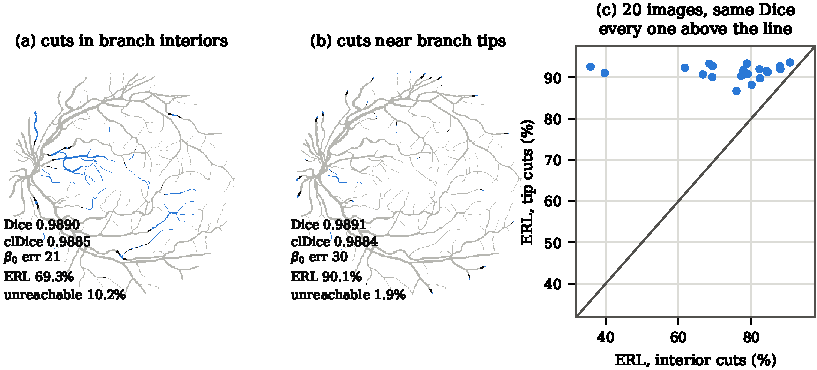
\includegraphics[width=\linewidth]{figures/fig1_case_set.pdf}
  \caption{The same mask, cut \csCuts{} times with the same discs at the same
  calibre; only the position along the branch differs. Black is the tissue
  removed, blue is what it cut off from the tree. (a) interiors, (b) tips ---
  both read Dice \csDice. (c) every one of \csImages{} images sits above the
  diagonal.}
  \label{fig:cases}
\end{figure}

\begin{table}[t]
  \centering
  \caption{A constructed case set on \csImages{} DRIVE test images,
  \csCuts{} cuts per arm. All four degraded arms delete the same area and
  post the same Dice. ``Unreachable'' is the quality anchor and is not
  derived from ERL. ERL convention: split\,/\,pixels\,/\,full.}
  \label{tab:cases}
  % tab1_case_set.tex -- GENERATED by exp/paper_figures.py. Do not edit here;
% edit the script, or the measurement it reads. Source: exp/results/blind_spot.csv, 20 DRIVE test images, 30 cuts per arm, ERL convention split/pixels/full, nothing selected on any split.
\begin{tabular}{lccccc}
\toprule
Arm & Dice & clDice & $\beta_0$ err & ERL & Unreach. \\
\midrule
ground truth & 1.0000 & 1.0000 & 0.0 & 98.1\% & 0.5\% \\
erosion, off centreline & 0.9889 & 1.0000 & 0.0 & 98.1\% & 0.5\% \\
erosion, anywhere & 0.9889 & 0.9963 & 0.0 & 59.9\% & 0.5\% \\
cuts near tips & 0.9889 & 0.9877 & 30.2 & 91.4\% & 1.4\% \\
cuts in interiors & 0.9889 & 0.9878 & 19.8 & 74.0\% & 11.1\% \\
\bottomrule
\end{tabular}

\end{table}

% The single most quotable sentence in the paper is the Betti-0 reversal.
% Do not bury it: \csBettiMid{} < \csBettiTip{}, lower is better, so Betti-0
% prefers the arm that orphans \csUnreachMid\% of the tree over the one that
% orphans \csUnreachTip\%.  The mechanism is measured, not argued: only
% \csSplitsMid{} of \csCuts{} interior cuts add a component, because
% \csLoopsMid{} of them fall on loops created where arteries and veins cross
% in projection.

\TODO{state the reversal, then give the loop mechanism}
% Budget: ~130 words. One paragraph. This is the quotable one.
\FILL{8}

\section{The metric does not transfer off the shelf}
\label{sec:reference}
% BUDGET: 3/4 column + Table 2.  This is the part nobody else has.
%
% Two defects, both found by RUNNING the reference package (version
% \refVersion), not by reading it:
%   (a) an undocumented connectivity assumption: their loop walks only the
%       component containing the first node of each label.  Harmless in 3D
%       connectomics, catastrophic here -- \refUnwalkedA\% of covered
%       skeleton went unmeasured on one image.
%   (b) fragment length is not well defined: a 3-px L corner reads
%       \refCornerA{} or \refCornerB{} depending on the order its nodes were
%       listed, because the walk keeps every diagonal of a DFS tree.
% Also worth one sentence: the merge penalty, the most distinctive half of
% the original metric, never fires here, because the retinal ground truth is
% a single connected object.

\TODO{section 3 prose}
% Budget: ~300 words. Defect (a), defect (b), one sentence on the merge term.
\FILL{9-11}

\begin{table}[t]
  \centering
  \caption{Running \texttt{segmentation-skeleton-metrics} \refVersion{} on
  DRIVE. Their loop measures only the component containing each label's
  first node; the rest of the covered skeleton is silently dropped.
  }
  \label{tab:reference}
  % tab2_reference.tex -- GENERATED by exp/paper_figures.py. Do not edit here;
% edit the script, or the measurement it reads. TRANSCRIBED from stage-report/erl_reference.md (run of segmentation-skeleton-metrics 5.9.5 on 2026-09-05); the package is not installed here, so this table is NOT recomputed.
\begin{tabular}{lccc}
\toprule
Image & Covered skeleton & Their ERL & After relabelling \\
      & not measured     & (px)      & (px) \\
\midrule
01 & 97.8\% & 21.81 & 6394.21 \\
02 & 13.7\% & 7874.06 & 6929.71 \\
03 & 95.3\% & 33.47 & 1033.64 \\
\bottomrule
\end{tabular}

\end{table}

\section{A specification, and what it costs to ignore it}
\label{sec:specification}
% BUDGET: 3/4 column.  No table if space is tight -- the numbers carry it.
%
%   axis 1  denominator: covered skeleton only, or the whole ground truth
%   axis 2  fragment length: pixel count, 8-neighbour edge weights, diameter
%   axis 3  does a bridged gap split a run
%
% Crossed on \specArms{} arms x \specSeeds{} seeds, the spread is
% \specSpreadLo--\specSpreadHi{} points, against a largest honest effect of
% \specHonest{} points in the same repository.  The ranking does not survive
% the choice: Spearman \specRho{}, largest rank move \specMove{}.
%
% Then the scaling rule, which is what makes this a specification rather
% than a complaint: the spread is bounded by how much skeleton the
% prediction fails to cover, so it shrinks on easy data
% (VessMAP \txVessmapLo--\txVessmapHi{} points at \txVessmapCov\% coverage
% against STARE's \txStareLo--\txStareHi{} at \txStareCov\%).  Read backwards:
% a paper reporting ERL on easy data hides less disagreement.

\TODO{section 4 prose}
% Budget: ~300 words (3/4 column minus the specification list below).
\FILL{12-14}

\begin{figure}[t]
  \centering
  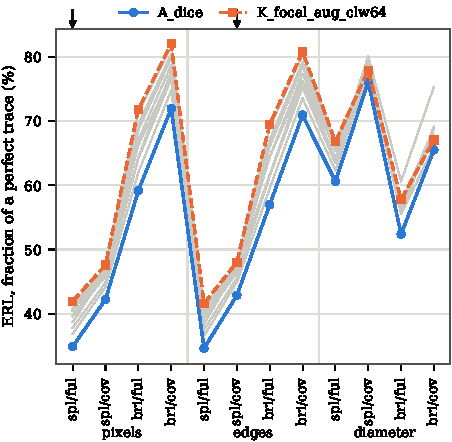
\includegraphics[width=\linewidth]{figures/fig2_conventions.pdf}
  \caption{One set of predictions on DRIVE (\specArms{} arms,
  \specSeeds{} seeds), read under each of the twelve legal cells. Grey is every
  arm; two are named. The shaded columns mark the cell the reference implementation
  computes (\texttt{split/edges/covered}) and the one this literature most often
  implements (\texttt{split/pixels/full}). Each arm spans
  \specSpreadLo--\specSpreadHi{} points without anything about the model, the
  data, the threshold or the checkpoint changing, and the arms cross: Spearman
  $\rho = \specRho$ between the two extreme cells, largest rank move
  \specMove{} of \specArms.}
  \label{fig:conventions}
\end{figure}

\begin{figure}[t]
  \centering
  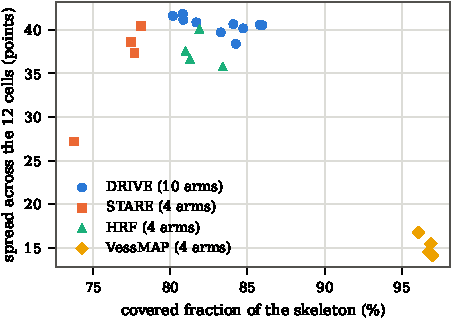
\includegraphics[width=\linewidth]{figures/fig3_coverage.pdf}
  \caption{The disagreement is not a constant. It is bounded by how much
  ground-truth skeleton the prediction fails to cover, so it collapses on easy
  data: VessMAP spans only \txVessMAPLo--\txVessMAPHi{} points at
  \txVessMAPCov\% coverage, against STARE's \txSTARELo--\txSTAREHi{} at
  \txSTARECov\%. Read backwards, a paper reporting ERL on easy data hides less
  disagreement than one on hard data.}
  \label{fig:coverage}
\end{figure}

\begin{table}[t]
  \centering
  \caption{Per-arm spread across the twelve cells, DRIVE, \specSeeds{} seeds.
  The largest honest effect any published topology loss produces in our own
  experiments, read at each arm's own dev-optimal threshold, is
  \specHonest{} points.}
  \label{tab:spread}
  \small
  % tab3_spread.tex -- GENERATED by exp/paper_figures.py. Do not edit here;
% edit the script, or the measurement it reads. Source: exp/results/heldout/erl_spec*.csv, recomputed and asserted equal to exp/results/erl_spec.txt by the selftest.
\begin{tabular}{lcccl}
\toprule
Arm & Lowest & Highest & Spread & Highest cell \\
\midrule
\texttt{H\_aug\_w64\_d5} & 38.4\% & 80.2\% & 41.8 & split/diameter/covered \\
\texttt{A\_dice} & 34.6\% & 76.2\% & 41.6 & split/diameter/covered \\
\texttt{H\_aug} & 36.5\% & 77.7\% & 41.1 & split/diameter/covered \\
\texttt{H\_aug\_clw2} & 37.5\% & 78.3\% & 40.9 & split/diameter/covered \\
\texttt{H\_aug\_clw16} & 39.3\% & 79.9\% & 40.7 & bridged/pixels/covered \\
\texttt{H\_aug\_clw64} & 41.1\% & 81.7\% & 40.6 & bridged/pixels/covered \\
\texttt{K\_focal\_aug\_clw64} & 41.6\% & 82.1\% & 40.5 & bridged/pixels/covered \\
\texttt{K\_focal\_aug\_clw32} & 40.3\% & 80.5\% & 40.2 & bridged/pixels/covered \\
\texttt{H\_aug\_clw8} & 39.4\% & 79.1\% & 39.7 & split/diameter/covered \\
\texttt{A\_dice\_clw64} & 40.1\% & 78.5\% & 38.4 & split/diameter/covered \\
\bottomrule
\end{tabular}

\end{table}


\noindent\textbf{The specification.} Report, next to every ERL number:
\begin{enumerate}
  \item the denominator, the length rule, and the splitting rule;
  \item the coverage, so the reader can convert between denominators;
  \item the amount of predicted foreground \NOTE{ERL is gameable by painting};
  \item which annotator was taken as ground truth \NOTE{5x on STARE};
  \item that the merge term does not fire, and that crossings are unpriced.
\end{enumerate}

\section{Conclusion}
\label{sec:conclusion}
% BUDGET: 4 sentences.  State the limits honestly here rather than letting a
% reviewer find them: the case set is CONSTRUCTED, so it shows the metrics
% have no resolution for this difference, not that models fail this way
% often; the anchor speaks to the cut arms, not the erosion arms; DRIVE only.

\TODO{conclusion}
% Budget: 4 sentences, ~60 words.
\FILLS{15}{1-4}


% Page 5 content only.
% Everything below may spill onto the optional 5th page; technical content
% may not. Both sections are required by ISBI, even when nothing applies.
\section{Compliance with Ethical Standards}
\label{sec:ethics}
% REQUIRED by ISBI, whether or not approval was needed.  May sit on page 5.
This is a study of evaluation methodology conducted entirely on the public
DRIVE, STARE, HRF and VessMAP datasets \TODO{cite the ones you actually use},
for which no ethical approval was required.

\section{Acknowledgments}
\label{sec:acknowledgments}
% May sit on page 5.  A conflict-of-interest statement is expected here.
\TODO{funding, advisor, conflicts of interest}


\bibliographystyle{IEEEbib}
\bibliography{refs}

\end{document}
